\chap{ Memory Blocks}





\section{Part IV} 
The SRAM block in Figure 1 has a single port that provides the address for both read and write operations. For this part you will create a different type of memory module, in which there is one port for supplying the address for a read operation, and a separate port that gives the address for a write operation. Perform the following steps. \\
\\
    1. Create a new Quartus project for your circuit. To generate the desired memory module open the IP Catalog
and select the RAM: 2-PORT module in the Basic Functions > On Chip Memory category. As shown in
Figure 5, choose With one read port and one write port in the category called How will you be using
the dual port ram?\\
\\
Configure the memory size, clocking method, and registered ports the same way as Part II. As shown in
Figure 6 select I do not care (The outputs will be undefined) for Mixed Port Read-During-Write for
Single Input Clock RAM. This setting specifies that it does not matter whether the memory outputs the
new data being written, or the old data previously stored, in the case that the write and read addresses are
the same during a write operation.
\begin{figure}[h]
    \centering
    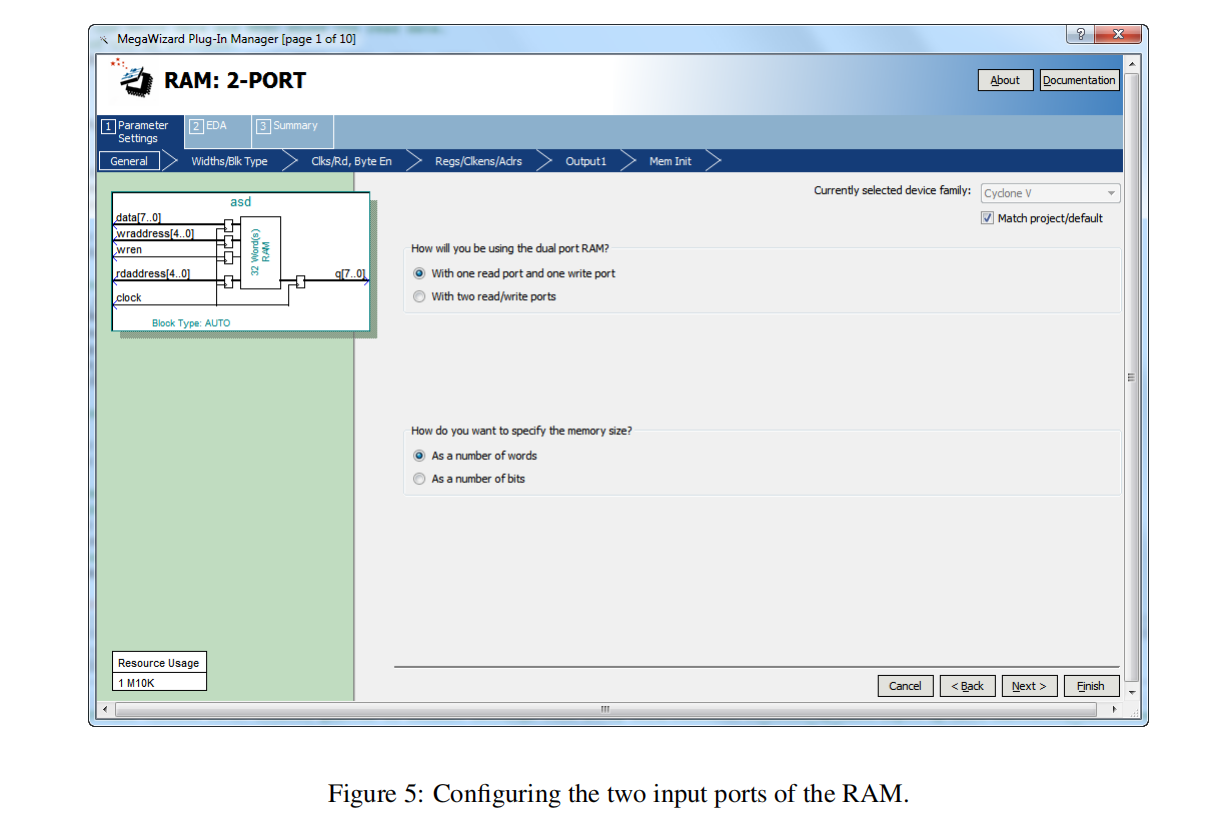
\includegraphics[scale = 0.4]{source/picture/Lab8/bai8_minhhoa1.png}
\end{figure}
\newpage

\begin{figure}[h]
    \centering
    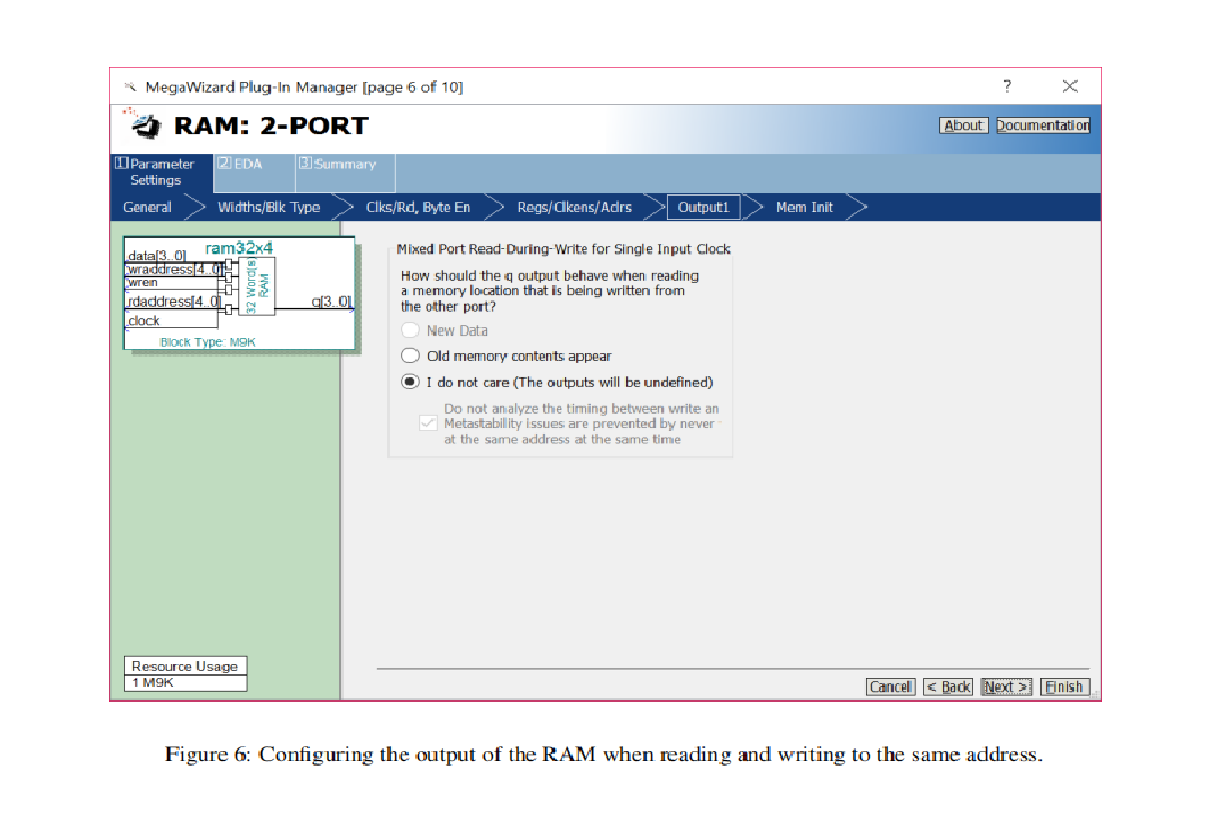
\includegraphics[scale = 0.4]{source/picture/Lab8/bai8_minhhoa2.png}
\end{figure}
Figure 7 shows how the memory words can be initialized to specific values. It makes use of a feature that
allows the memory module to be loaded with data when the circuit is programmed into the FPGA chip.
As shown in the figure, choose the setting Yes, use this file for the memory content data, and specify
the filename ram32x4.mif. An example of a MIF file is provided in Figure 8. You can also learn about the
format of a memory initialization file (MIF) by using the Quartus Help. You will need to create a MIF file
like the one in Figure 8 to test your circuit. Finish the Wizard and then examine the generated memory
module in the file ram32x4.v.

\begin{figure}[h]
    \centering
    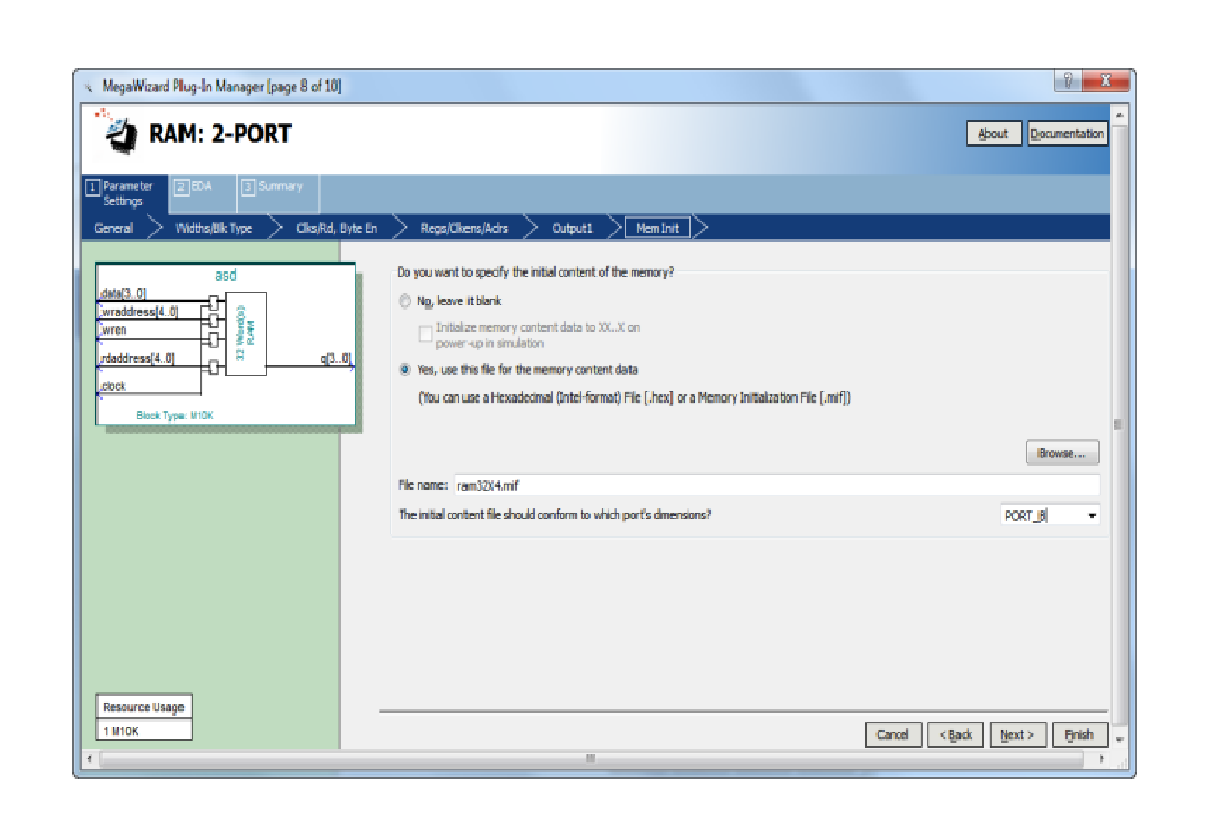
\includegraphics[scale = 0.4]{source/picture/Lab8/bai8_minhhoa3.png}
\end{figure}
\newpage
\begin{figure}[h]
    \centering
    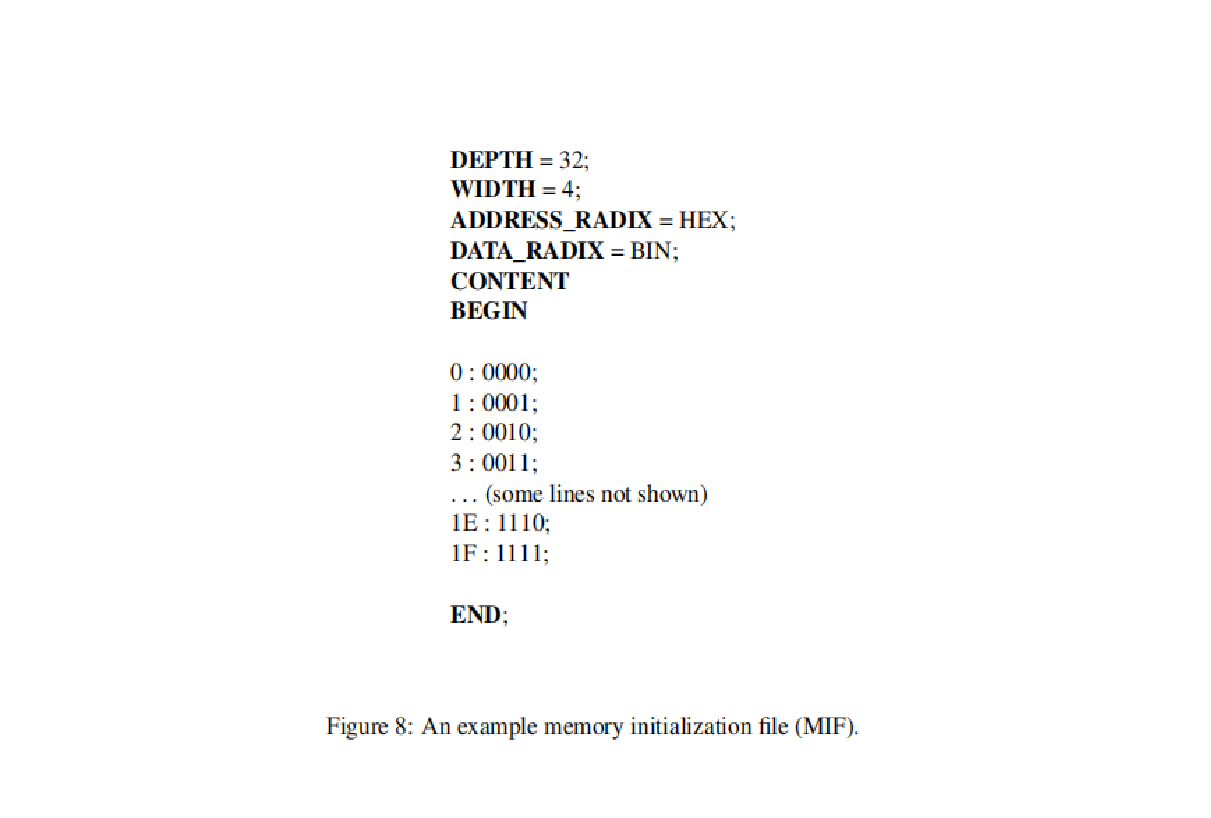
\includegraphics[scale = 0.5]{source/picture/Lab8/bai8_minhhoa4.png}
\end{figure}
2. Write a Verilog file that instantiates your dual-port memory. To see the RAM contents, add to your design a capability to display the content of each four-bit word (in hexadecimal format) on the 7-segment display 6-HEX0. Use a counter as a read address, and scroll through the memory locations by displaying each word for about one second. As each word is being displayed, show its address (in hex format) on the 7-segment displays HEX3-2. Use the 50 MHz clock, CLOCK50, and use KEY0 as a reset input. For the write address and corresponding data use switches SW8-4 and SW3-0. Show the write address on HEX5-4 and show the write data on HEX1. Make sure that you properly synchronize the slide switch inputs to the 50 MHz clock signal.\\
\\
3. Test your circuit and verify that the initial contents of the memory match your ram32x4.mif file. Make sure
that you can independently write data to any address by using the slide switches.\\

\begin{figure}[h]
    \centering
    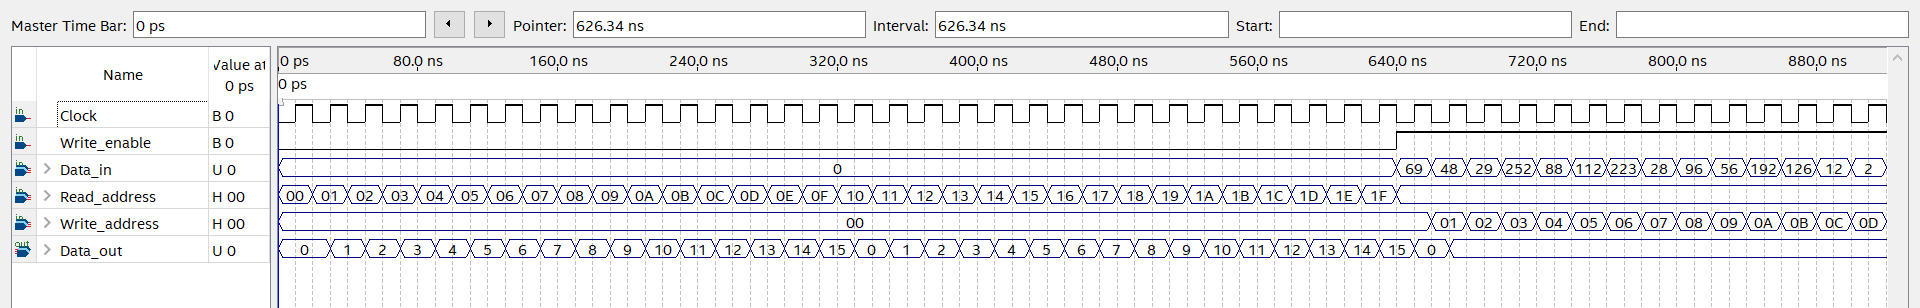
\includegraphics[scale = 0.4]{source/picture/Lab8/simulation_1.png}
    \caption{Simulation 1}
\end{figure}
\newpage
\begin{figure}[h]
    \centering
    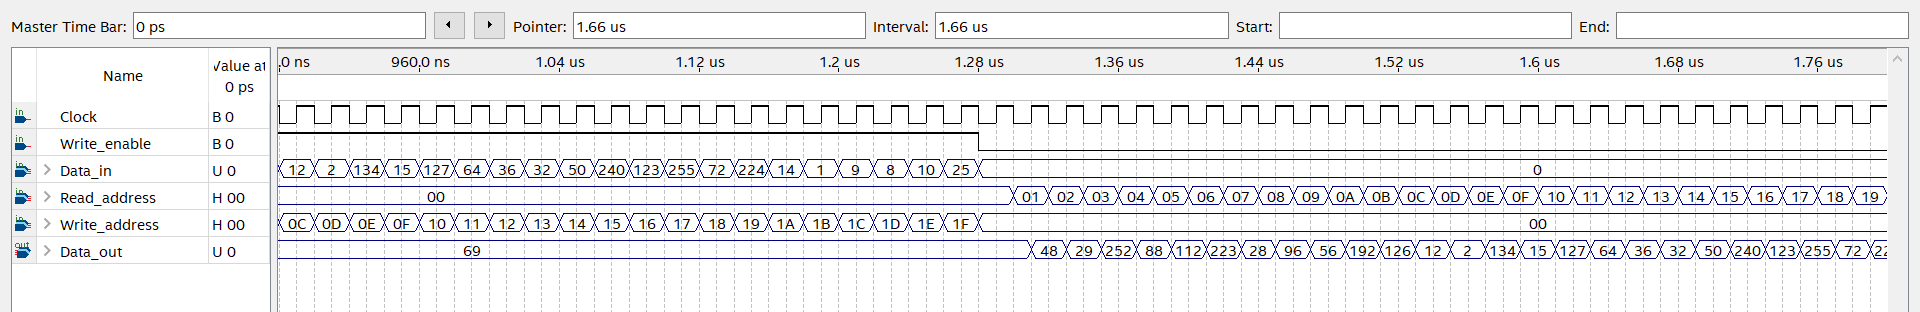
\includegraphics[scale = 0.4]{source/picture/Lab8/simulation_2.png}
    \caption{Simulation 2}
\end{figure}
\begin{figure}[h]
    \centering
    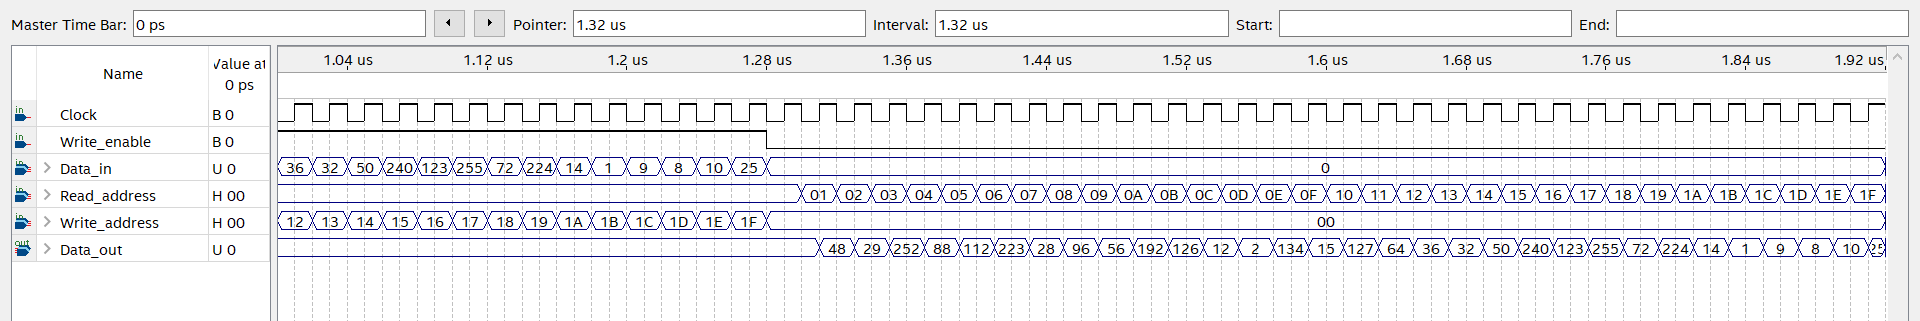
\includegraphics[scale = 0.4]{source/picture/Lab8/simulation_3.png}
    \caption{Simulation 3}
\end{figure}
The following is the code of ram 32x4.mif file which is initialized for the memory.
\begin{lstlisting}[language=Verilog]
DEPTH = 32;
WIDTH = 4;
ADDRESS_RADIX = HEX;
DATA_RADIX = BIN;
CONTENT
BEGIN
0  : 0000;
1  : 0001;
2  : 0010;
3  : 0011;
4  : 0100;
5  : 0101;
6  : 0110;
7  : 0111;
8  : 1000;
9  : 1001;
A  : 1010;
B  : 1011;
C  : 1100;
D  : 1101;
E  : 1110;
F  : 1111;
10 : 0000;
11 : 0001;
12 : 0010;
13 : 0011;
14 : 0100;
15 : 0101;
16 : 0110;
17 : 0111;
18 : 1000;
19 : 1001;
1A : 1010;
1B : 1011;
1C : 1100;
1D : 1101;
1E : 1110;
1F : 1111;
END;

\end{lstlisting}
